\documentclass[11pt]{article}
\usepackage[margin=1in]{geometry}                % See geometry.pdf to learn the layout options. There are lots.
\geometry{letterpaper}                   % ... or a4paper or a5paper or ... 
%\geometry{landscape}                % Activate for for rotated page geometry
%\usepackage[parfill]{parskip}    % Activate to begin paragraphs with an empty line rather than an indent


\usepackage{graphicx}
\usepackage{amssymb}
\usepackage{epstopdf}
\usepackage{wrapfig}
\usepackage[margin=1in,font=small,labelfont=bf,
               labelsep=colon]{caption}

\DeclareGraphicsRule{.tif}{png}{.png}{`convert #1 `dirname #1`/`basename #1 .tif`.png}



\title{ALDEx2: ANOVA-Like Differential Expression tool for compositional data}
\author{Greg Gloor}
\date{\today}                                           % Activate to display a given date or no date

\begin{document}
\maketitle
\tableofcontents
%\listoffigures
%\listoftables
\section{Why another package?}
Fundamentally, many high throughput sequencing approaches generate similar data: reads are mapped to features in each sample, these features are normalized, then statistical difference between the features composing each group or condition is calculated.  The standard statistical tools used to analyze RNA-seq, ChIP-seq, 16S rRNA gene sequencing, metagenomics, etc.\ are fundamentally different for each approach  despite the underlying similarity in the data structures. ALDEx2 provides a simple consistent framework for data analysis that encompasses all these experimental designs by modelling the data as proportions rather than counts.

\section{Introduction}
This guide provides an overview of the R package ALDEx version 2 (ALDEx2) for differential abundance analysis of proportional data. The package was developed specifically for multiple-organism RNA-Seq data generated by high-throughput sequencing platforms (meta-RNA-Seq)\cite{macklaim:2013}, but testing showed that it performed very well with traditional RNA-Seq datasets, 16S rRNA gene variable region sequencing and selective growth-type (SELEX) experiments\cite{fernandes:2013,fernandes:2014}. In principle, the analysis method should be applicable to nearly any type of data that is generated by high-throughput sequencing that generates tables of per-feature counts for each sample: in addition to the examples outlined above this would include  ChIP-Seq or metagenome sequencing. We will be including examples for application on these types of problems as we move forward.

Versions of the ALDEx2 package greater than 2.0.7 are modular and are suitable for the comparison of many different experimental designs. They are named ALDEx2m. This is achieved by exposing the underlying values to make it possible for anyone to add the specific R code for their experimental design --- a guide to these values is in Section \ref{clr}. If there are only two replicates in one condition ALDEx2 can give the same information as ALDEx version 1. 

ALDEx2 estimates per-feature technical variation within each sample using Monte-Carlo instances drawn from the Dirichlet distribution. This distribution maintains the proportional nature of the data. ALDEx2 uses the centred log-ratio (clr) transformation that ensures the data are scale invariant and sub-compositionally coherent\cite{Aitchison:1986}. The scale invariance property removes the need for a between sample data normalization step since the data are all placed on a consistent numerical co-ordinate. The sub-compositional coherence property ensures that the answers obtained are consistent when parts of the dataset are removed (e.g., removal of rRNA reads from  RNA-seq studies or rare OTU species from 16S rRNA gene amplicon studies). All feature abundance values are expressed relative to the geometric mean abundance of all features in a sample. This is conceptually similar to a quantitative PCR where abundances are expressed relative to a standard: in the case of the clr transformation, the standard is the per-sample geometric mean abundance. See Aitchison (1986)\cite{Aitchison:1986} for a complete description, or the lecture notes from CoData5\cite{aitchisonconcise}.

\section{Installation}
Download the most current non-test version of ALDEx2. Versions that are noted as ALDEx2t are test versions and may not be reliable or documented. Do not unzip or untar the file. Inside an R environment type the following  (replacing the /path/to with the path to the file on your computer):
\begin{verbatim}
install.packages("/path/to/ALDEx2m_2.0.7.1.tar.gz", repos=NULL, type="source")
\end{verbatim}
At the present, ALDEx2 will run with only the base R packages. It has been tested with version R version 3, but should run on version 2.12 onward. If the package \texttt{multicore} is present, ALDEx2 will make use of it.

\section{Quick example with `selex' example data and 2 groups:}
Case study a growth selection type experiment\cite{mcmurrough:2014}: This section contains an analysis of a dataset collected where a single gene  library was made that contained 1600 sequence variants at 4 codons in the sequence. These variants were cloned into an expression vector at equimolar amounts. The wild-type version of the gene conferred resistance to a topoisomerase toxin. Seven independent growths of the gene library were conducted under selective and non-selective conditions and the resulting abundances of each variant was read out by sequencing a pooled, barcoded library on an Illumina MiSeq\cite{mcmurrough:2014}. The data table is included as selex\_table.txt in the package. In this data table, there are 1600 features and 14 samples. The analysis takes approximately 2 minutes and memory usage tops out at less than 1Gb of RAM on a mobile i7 class processor.  The commands used for modular ALDEx are presented below:

\begin{verbatim}
# load the library
library(ALDEx2)  

# load the included selex dataset
data(selex)  

# set comparison groups
# a vector of conditions with the order of the samples in the input counts table
conds <- c(rep("NS", 7), rep("S", 7))  

###############
# Single command approach
# this is identical to ALDEx2 versions before 2.0.7
# test: t = Welch's t + Wilcoxon, glm = glm + Kruskal-Wallace
x <- aldex(selex, mc.samples=128, test="t", effect=TRUE, 
     include.sample.summary=FALSE, verbose=FALSE)
# plot the data
# types: MA, MW
aldex.plot(x, type="MA", test="welch")
aldex.plot(x, type="MW", test="welch")
##############

###############
# Modular approach that exposes the underlying intermediate data
# the simple approach just calls aldex.clr, aldex.ttest, aldex.effect in turn
# and then merges the data into one object

# generate instances of the centred log-ratio transformed values
# three inputs: counts table, number of Monte-Carlo instances, print steps
# this is fast
x <- aldex.clr(selex, mc.samples=128, verbose=TRUE)  

# perform the Welch's t and Wilcoxon rank test
# this test should be used for two condition tests
# three inputs: the aldex object from aldex.clr, vector of conditions, paired test or not
x.tt <- aldex.ttest(x, conds, paired.test=TRUE)  

# perform the glm and Kruskal Wallace tests
# this test should be used for one-way ANOVA of more than two conditions 
# two inputs: the aldex object from aldex.clr, vector of conditions
# this is slow!
x.glm <- aldex.glm(x, conds)  

# estimate effect size and the within and between condition values 
# this is only for use with two conditions
# this step is required for plotting
# three inputs: the aldex object from aldex.clr, vector of conditions, include values for 
# all samples or not, print steps
x.effect <- aldex.effect(x, conds, include.sample.summary=FALSE, verbose=TRUE) 

# merge the data
x.all <- data.frame(x.tt, x.glm, x.effect)

# plot the data
# tests: welch, wilcox, glm, kruskal
# types: MA, MW
aldex.plot(x.all, type="MA", test="welch")
aldex.plot(x.all, type="MW", test="welch")
################
\end{verbatim}
\begin{figure}[!h]
\begin{center}
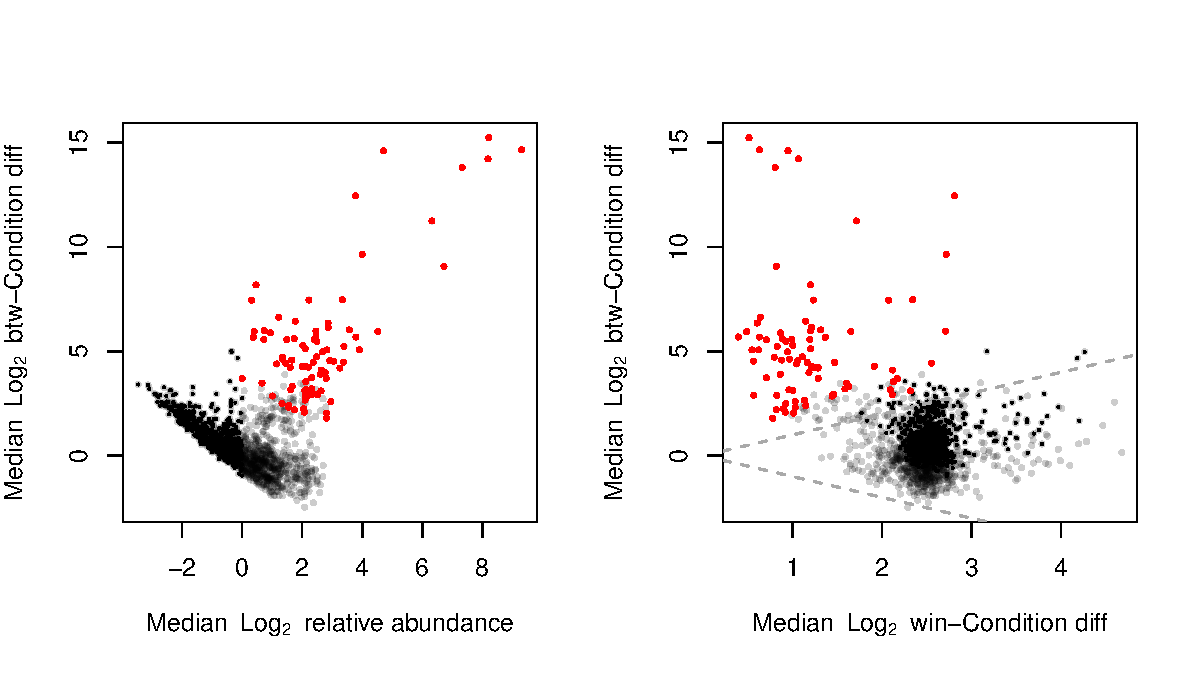
\includegraphics[width=6in]{/Users/ggloor/git/ALDEx2/manual/aldex_plot.pdf}
\caption{Output from \texttt{aldex.plot} function. The left panel is the MA plot, the right is the MW plot. In both plots red represents features called as differentially abundant with q $<0.1$; grey are abundant, but not non-differentially abundant; black are rare, but not differentially abundant.}
\label{selex}\vspace{-0.8cm}
\end{center}
\end{figure}

\newpage

\begin{verbatim}
# examine the data
head(x.all)
               we.ep      we.eBH        wi.ep      wi.eBH       kw.ep
A:D:A:D 4.030100e-01 0.630807054 0.2393830128 0.437328198 0.215320607
A:D:A:E 1.154636e-01 0.347445969 0.0409018065 0.157258414 0.037453159
A:E:A:D 8.987974e-05 0.003290767 0.0005827506 0.008207592 0.001745119
            kw.eBH       glm.ep      glm.eBH  rab.all rab.win.NS rab.win.S
A:D:A:D 0.39327439 3.610615e-01 5.235822e-01 1.424946   1.308861  2.453840
A:D:A:E 0.14865903 8.122652e-02 1.922925e-01 1.712300   1.497671  4.233156
A:E:A:D 0.02457865 7.736602e-08 3.354920e-06 3.974840   1.411636 11.021544
        diff.btw diff.win    effect      overlap
A:D:A:D 1.122613 1.729108 0.4710433 0.2672607019
A:D:A:E 2.730902 2.381348 1.0348739 0.1358577816
A:E:A:D 9.642872 2.850081 3.4290684 0.0001566327
\end{verbatim}

ALDEx2 returns expected values for summary statistics. It is important to note that ALDEx uses Bayesian sampling from a Dirichlet distribution to estimate  the underlying technical variation. This is controlled by the number of \texttt{mc.samples}, in practice we find that setting this to 128 is sufficient for most cases as ALDEx2 is estimating the expected value of the distributions\cite{fernandes:2014}. The user is cautioned that the number of features called as differential will vary somewhat between runs because of the sampling procedure. Only features with values close to the chosen significance cutoff will vary between runs. 

In the list below, the \texttt{aldex.ttest} function returns the values highlighted with $\ast$, the \texttt{aldex.glm} function returns the values highlighted with $\circ$, and the \texttt{aldex.effect} function returns the values highlighted with $\diamondsuit$. 

\begin{itemize}
  \setlength{\itemsep}{1pt}
  \setlength{\parskip}{4pt}
  \setlength{\parsep}{0pt}
\item[$\ast$] we.ep - Expected P value of Welch's t test 
\item[$\ast$] we.eBH - Expected Benjamini-Hochberg corrected P value of Welch's t test 
\item[$\ast$] wi.ep - Expected P value of Wilcoxon rank test 
\item[$\ast$] wi.eBH - Expected Benjamini-Hochberg corrected P value of Wilcoxon test 
\item[$\circ$] kw.ep - Expected P value of Kruskal-Wallace  test 
\item[$\circ$] kw.eBH - Expected Benjamini-Hochberg corrected P value of Kruskal-Wallace  test 
\item[$\circ$] glm.ep - Expected P value of glm test 
\item[$\circ$] glm.eBH - Expected Benjamini-Hochberg corrected P value of glm test 
\item[$\diamondsuit$] rab.all - median clr value for all samples in the feature
\item[$\diamondsuit$] rab.win.NS - median clr value for the NS group of samples
\item[$\diamondsuit$] rab.win.S - median clr value for the S group of samples
\item[$\diamondsuit$] rab.X1\_BNS.q50 - median expression value of features in sample X1\_BNS if \texttt[include.item.summary=TRUE]
\item[$\diamondsuit$] dif.btw - median difference in clr values between S and NS groups
\item[$\diamondsuit$] dif.win - median of the largest difference in clr values within S and NS groups
\item[$\diamondsuit$] effect - median effect size:  diff.btw / max(dif.win) for all instances
\item[$\diamondsuit$] overlap - proportion of effect size that overlaps 0 (i.e. no effect)
\end{itemize}

The built-in aldex.plot function described above will usually be sufficient. The example and plot below shows a plot that incorporates all the significance tests into one plot.

\begin{verbatim}
# identify which values are significant in all tests
found.by.all <- which(x.all$we.eBH < 0.05 & 
 x.all$wi.eBH < 0.05 & x.all$glm.eBH < 0.05 & x.all$kw.eBH < 0.05)

# identify which values are significant in fewer than all tests
found.by.one <- which(x.all$we.eBH < 0.05 | 
 x.all$wi.eBH < 0.05 | x.all$glm.eBH < 0.05 | x.all$kw.eBH < 0.05)

# plot the within and between variation of the data
plot(x.all$diff.win, x.all$diff.btw, pch=19, cex=0.3, col=rgb(0,0,0,0.3),
 xlab="Difference within", ylab="Difference betweenn")
points(x.all$diff.win[found.by.one], x.all$diff.btw[found.by.one], pch=19, 
 cex=0.5, col=rgb(0,0,1,0.5))
points(x.all$diff.win[found.by.all], x.all$diff.btw[found.by.all], pch=19, 
 cex=0.5, col=rgb(1,0,0,1))
abline(0,1,lty=2)
abline(0,-1,lty=2)
\end{verbatim}

\begin{figure}[!h]
\begin{center}
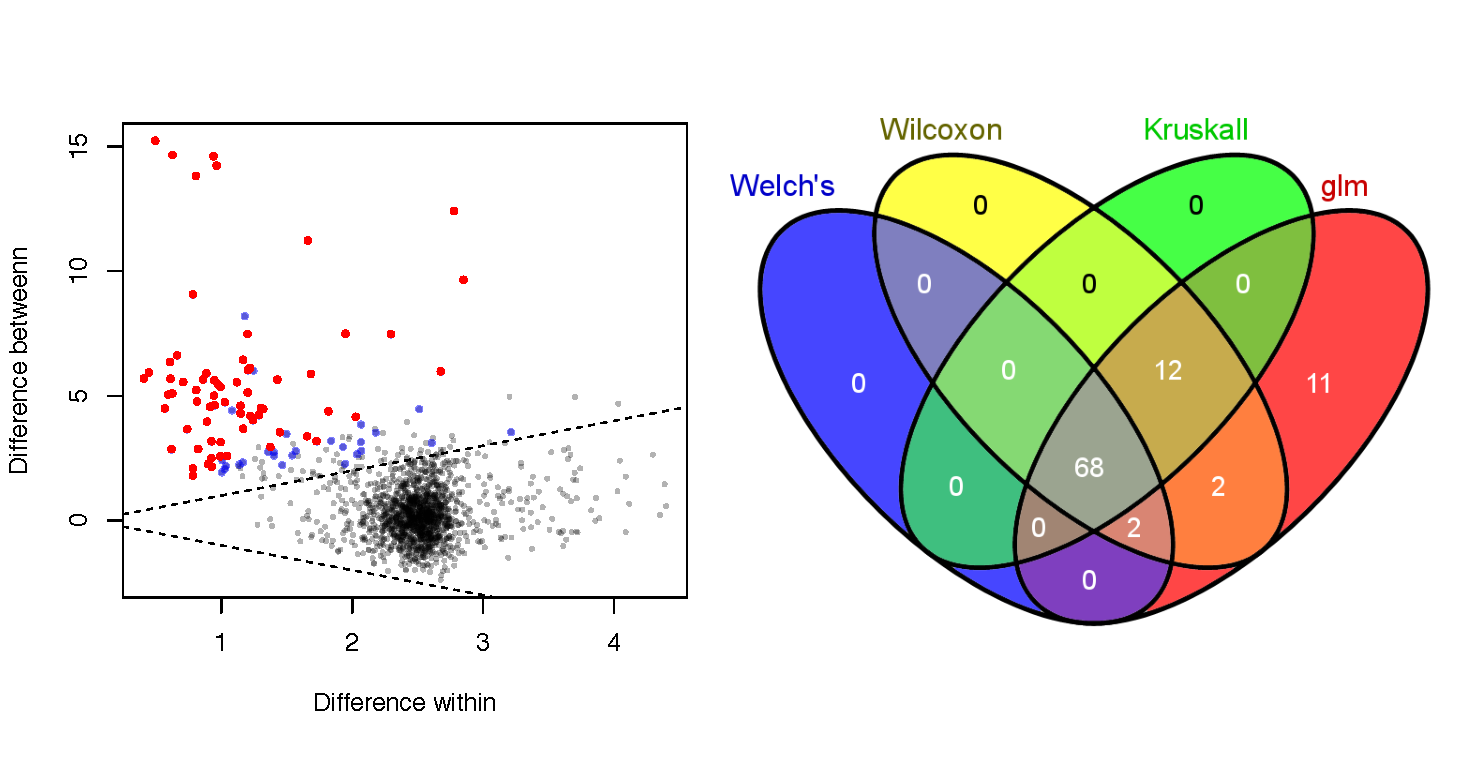
\includegraphics[width=6in]{/Users/ggloor/git/ALDEx2/manual/selex_comparison.pdf}
\caption{Differential abundance in the selex dataset using the Welch's t-test, Wilcoxon rank test, Kruskall-Wallace test or  glm function. There were 68 features identified by all tests shown in red. Features identified by three or fewer tests are shown in blue dots.  Non-significant features represent rare features if black and abundant features if grey dots. The breakdown is shown in the Venn diagram using the Venny web tool\cite{oliveros:2007}. }
\label{selex}\vspace{-0.8cm}
\end{center}
\end{figure}

\newpage

\section{General information}
%The underpinnings of ALDEx and ALDEx2 are explained two papers\cite{fernandes:2013, fernandes:2014}. The purpose of these instructions is an explanation of how to use ALDEx2. This version of ALDEx is modular, providing access to the underlying centre log-ratio transformed instances. This approach allows investigators to write their own functions for their individual experimental designs. Examples of all current functions, along with some basic R pitfalls in setting up the required input tables are included below. The authors expect that there is a current working installation of the R statistical programming language that is properly installed, and that the user has a basic understanding of it. ALDEx2 and has been tested on R version 3.

The authors appreciate bug reports or suggestions for improvements to the package, and would encourage users to incorporate additional modular functions for more complex experimental designs.

\subsection{Differences with the version in the 2013 Fernandes et al PLoS ONE paper}  

\begin{table}
\begin{center}
\caption{Time to complete a dataset in seconds between exhaustive (2.0.5) and random (2.0.6) versions. The sample sizes are rows x columns by samples.}
\begin{tabular}{cccc}

version & dataset & DMC  &  time\\\hline
2.0.5  &  selex  &  128  &  107.246\\
2.0.5  &  selex  &  128  &  108.601\\
2.0.6  &  selex  &  128  &  92.718\\
2.0.6  &  selex  &  128  &  94.241\\
2.0.5  &  bottomly  &  128  &  1198.984   \\
2.0.6  &  bottomly  &  128  &  919.952\\
2.0.5  &  16S-tag  &  16  &  DNF\\
2.0.6  &  16S-tag,vag (133x133x7239)  &  16  &  542.607\\
2.0.6  &  16S-tag,oral (316x312x23393)  &  16  &  4571.960\\
\end{tabular}
\label{exvsra}
\end{center}
\end{table}

\begin{itemize}

\item ALDEx2  requires substantially less memory and can accordingly be run over even larger datasets than the original version of ALDEx. ALDEx v1.0.4 is available at: \begin{verbatim}https://github.com/ggloor/ALDEx2/blob/master/ALDEx_1.0.4.tar.gz\end{verbatim} No further changes other than bug fixes are expected for that version. 

\item ALDEx2 uses standard statistical tests to determine p values and false discovery rates. The modular version described here can be easily adapted to any study design. ALDEx2 will give results with only 2 replicates, however, only the effect and overlap statistics are meaningful under these conditions: \emph{p values and Benjamini-Hochberg values are not reliable with only 2 conditions}.

\item Note: ALDEx2 removes all features that have 0 reads mapped in all samples.
\end{itemize}

\subsection{New in version 2.0.7 and greater:} The program is now modular and provides access to the underlying instances of the clr values calculated from the Dirichlet Monte-Carlo replicates. Arianne Albert wrote the glm and Kruskal-Wallice module for one-way ANOVA and the correlation module. The program can now use parallel processing through the multicore package if present. Matt Links provided this code. It will run without the package, but somewhat slower. 

\begin{wrapfigure}{r}{0.6\textwidth}\vspace{-2cm}
\begin{center}
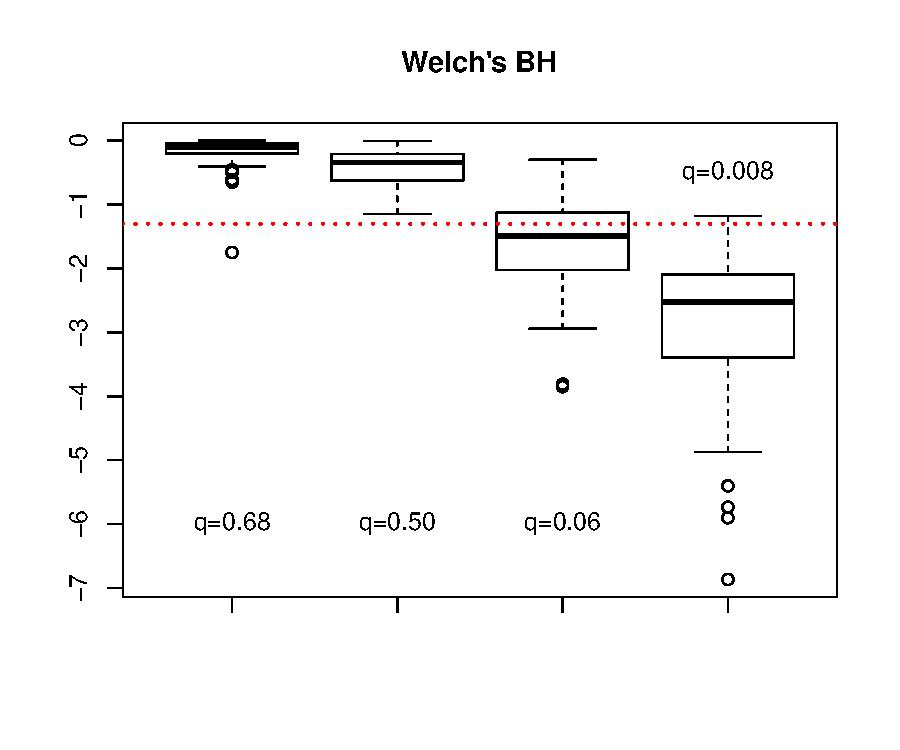
\includegraphics[width=0.6\textwidth]{/Users/ggloor/git/ALDEx2/manual/DirvsBH.pdf}
\vspace{-1cm}
\caption{The effect of modelling the data as proportions using Monte-Carlo instances drawn from a Dirichlet distribution and clr transformation on corrected p values. The typical experiment has many replicates and few samples, thus the technical variation in the data is modelled poorly. Shown here are the distribution of Benjamini-Hochberg corrected p values (q value) for 128 Monte-Carlo instances. Only the last one is reported as significant by ALDEx2 (expected q value indicated above the bars), yet some inferred technical replicates of each feature would give significant q values. Taking the expected value of the distribution rather than a single point estimate ensures that only features that exhibit significance consistently are identified as significantly different. The  red line shows the location of q\ $=0.05$. }
\label{dirvsbh}
\end{center}\vspace{-2cm}
\end{wrapfigure}
\newpage
\subsection{New in version 2.0.6 and greater:} The major memory constraint has been largely removed. It was caused by an all vs. all approach for the comparison of vectors used to generate the within and between group difference values, and for the effect size calculation. The exhaustive approach is taken up to the point where the vectors exceed a length of 10000. After that limit, the vector is randomly sampled to 10000 instance. Testing has found that the values are identical to the second decimal place with the original approach for large datasets. The differences in speed are given in Table \ref{exvsra}.

\section{Modelling the data as proportions}
For high-throughput sequencing experiments, including RNA-seq, individual sequence reads are assigned to genes or genomic features and the typical output is a table of counts per feature. Reads assigned to these features have several sources of variation: technical variation, biological variation within a condition, biological variation between conditions and unexplained variation. The consensus view in the literature is that the underlying variation is best explained by the modelling the pooled variation of  features with a given condition using negative binomial distribution\cite{Anders:2013aa}. 

We take a different approach with ALDEx and ALDEx2. First, we do not assume the technical variation of the features in a given sample share any underlying distribution. Second, we model the reads as proportions  of the data available rather than as counts. The proportional nature of the data is a result of the large but finite number of reads available from a next-generation sequencing run. See Fernandes et al.\cite{fernandes:2013} for a discussion of the advantages of modelling the data in this way. 

In brief, we we use Baysian techniques to infer the underlying technical variation in the read count proportions in a way that preserves the proportional nature of the data. This is done by sampling from a Dirichlet distribution, and results in a transformation of the observed read counts into a distribution of read counts. These distributions are centre log-ratio transformed following the advice of Aitchison\cite{Aitchison:1986} for dealing with proportional data. This has three effects. First, the abundance values for each sample are centred on their geometric mean abundance levels. Second, the data now expose the same relationships regardless of how the input data is altered by subsetting. Third, the values become largely independent and can be dealt with as statistically independent features when there are large numbers of features. 

These clr transformed values are used for standard between-group statistical tests  followed by Benjamini-Hochberg corrections for false discovery rate. The expected value of the p and q scores is returned to the user. This ensures that features that appear significant only because of random sampling error are weeded out, and that features that have significance that is robust to random sampling error are retained. An example for four features that have various significance scores is shown in Figure \ref{dirvsbh}. 

\section{Access to the underlying clr transformed Dirichlet Monte-Carlo instances}{\label{clr}
In the example from the quick start, x contains the initial instances of the clr values. 
\begin{verbatim}
# generate instances of the centred log-ratio transformed values
x <- aldex.clr(selex, mc.samples=128, verbose=TRUE)  

x is a list, where each list item is a matrix of features (rows) and 
clr-transformed Dirichlet Monte-Carlo instances (columns)

The list contents are named by the sample IDs: names(x)

Features (genes, OTUs, etc) are in rows in the matrix, and the number 
of features are the number of rows in any column, eg. number of features: 
     length(x[[1]][,1])
     
Instances are in the columns of the matrix, and the number of instances
are the number of columns in a row, eg. number of Monte-Carlo Dirichlet instances: 
     length(x[[1]][1,])
     
Identifiers for the features are the rownames of a sample: rownames(x[[1]])

\end{verbatim}

\newpage
\begin{wrapfigure}{R}[0mm]{0.4\textwidth}
\vspace{0cm}
\begin{center}
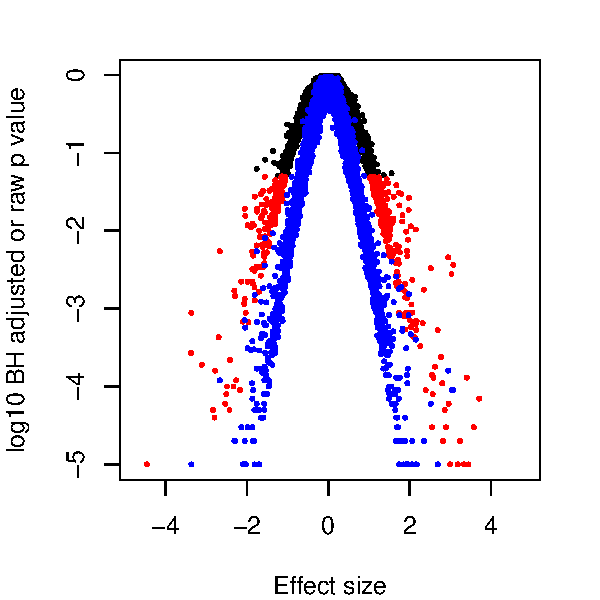
\includegraphics[width=0.4\textwidth]{/Users/ggloor/git/ALDEx2/manual/effect.pdf}
\caption{Plot showing correlation between effect size and p values. Black and red, show the plot for the Bottomly dataset, with black showing BH values $>0.05$ and red showing BH values $<= 0.05$. The blue dots show the plot for the selex dataset, with no distinction.}
\label{effect}
\end{center}\vspace{0cm}
\end{wrapfigure}

\section{The Relationship between Effect Size and P values} There is a very strong association between the effect size calculated as in Fernandes et al.\cite{fernandes:2013} and the Expected p value and the associated corrected p value. The effect size is determined by dividing the random vector of between-group differences by both random vectors of within-group differences, taking the larger of the two results, and taking the Expected value of the final vector. Effect size is thus a measure of the mean ratio of the difference between conditions and the maximum difference within conditions. When the sample size is small (say less than 4 in each condition)  the estimation of p values by either statistical test is less robust, it may be more appropriate to use an effect size cutoff of 1.5-2 and an overlap cutoff of 0.01 to identify differential features of interest\cite{fernandes:2013}. Conversely, when the number of samples is very large, the adjusted p value cutoffs will identify a large number of differential features because of the well-know relationship between sample size and power. However, it is likely that with extremely large sample sizes that statistical significance will over-estimate biological relevance when the effect size is small and the user is cautioned to use prudent effect size cutoffs\cite{Nakagawa:2007}.\
%pdf("/Users/ggloor/git/ALDEx2/manual/effect.pdf", height=4, width=4)
\begin{verbatim}pdf("effect.pdf", height=4, width=4)
plot(x.all$effect, log10(x.all$we.eBH),pch=19, 
  cex=0.3, xlab="Effect size", ylab="log10 BH adjusted or raw p value")
points(x.all$effect[x.all$we.eBH <0.05], 
  log10(x.all$we.BH[x.all$we.eBH <0.05]),pch=19, cex=0.3, col="red")
points(x.all$effect, log10(x.all$we.ep), 
  pch=19, cex=0.3,col="blue", xlab="Effect size", ylab="log10 p value")
dev.off()
\end{verbatim}

\newpage

\section{Grouping by Gene Function: SumFunctionsAitchison.R}
This section describes the approach used by Macklaim et al.\cite{macklaim:2013} to sum read counts across SEED, KEGG or COG functional groups. In brief: read counts are converted to proportions with an uninformative prior using the Aitchison mean\cite{Aitchison:1986}; these proportions are divided by the sequence length to normalize the read counts per unit length; the resulting values are divided by the sum of values for each sample to re-proportion the values so they sum to 1; each value is then multiplied by the original number of counts per sample; finally, values are summed by the group identifier. 

This approach is coded in the R function `SumFunctionsAitchison.R'. The function can be invoked on the command line as follows:
\begin{verbatim}
R CMD BATCH `--args in_filename out_filename 3' SumByAitchisonTransform.R log.txt 
\end{verbatim}
It requires three arguments, the input file name, the output file name, and the index of the first count column. The column structure of the input file should be as in the following example, where the first $n$ columns are ID columns, the next column is the length, followed by count columns. The final column must contain the grouping information.\\

\begin{tabular}{lllllll}
ID & length & count1 & count2 & ... & countn & Group\\\hline
RATOTCC & 1505 & 24 & 19 & ... & 341 & K00001\\
K02100 & 1463 & 3 & 0 & ... & 2 & K00001\\
\end{tabular}

\section{Contributors}
Andrew Fernandes wrote the original ALDEx code, and designed ALDEx2. Jean Macklaim found and squished a number of bugs, did  testing and did much of the validation. Matt Links incorporated ALDEx2 into a multicore environment. Adrianne Albert wrote the correlation and the one-way ANOVA modules. Andrew Fernandes, Jean Macklaim and Ruth Wong contributed to the Sum-FunctionsAitchison.R code. Greg Gloor is currently maintaining ALDEx2 and played roles in design and implementation.
%When the number of features is small  (less than about 200), or when they are homogeneous (for example modelled data without additional variance), or both, we find that lfdr is unable to fit to the data appropriately.  In this case we recommend using the q value instead. Note that when the number of features is less than 100 the qvalue may not be estimated accurately. 

%In any event, we caution the user to choose an fdr method that ensures that as few features as possible are in between the diagonal lines. In the example shown in Figure \ref{bottomly2} it can be seen that the tail-area based method (qval) (column 1) shows a number of features that have a larger difference within that difference between value, suggesting that this method is too inclusive. The Welch's t-test coupled with the density based false discovery method (lfdr, top right) appears to show a good balance between sensitivity and selectivity in this dataset.

 


%\begin{figure}[htbp]
%\begin{center}
%\includegraphics[width=4.5in]{/Users/ggloor/Documents/LaTeX/ALDEx/t-test_aldex/selex_hist.pdf}
%\caption{Histogram of p values in the Bottomly dataset. This dataset has low biological variability and the tail area-based q value would be a more powerful false discovery rate statistic in this instance.}
%\label{bottomly}
%\end{center}
%\end{figure}
\newpage
\bibliography{bibdesk_refs}
\bibliographystyle{plos2009}




\end{document}  